\documentclass{beamer}
\usetheme{CambridgeUS}
\usepackage{amssymb}

\AtBeginSection[]{
  \begin{frame}
  \vfill
  \centering
  \begin{beamercolorbox}[sep=8pt,center,shadow=true,rounded=true]{title}
    \usebeamerfont{title}\insertsectionhead\par%
  \end{beamercolorbox}
  \vfill
  \end{frame}
}

\AtBeginSubsection[]{
  \begin{frame}
  \vfill
  \centering
  \begin{beamercolorbox}[sep=8pt,center,shadow=true,rounded=true]{title}
    \usebeamerfont{title}\insertsubsectionhead\par%
  \end{beamercolorbox}
  \vfill
  \end{frame}
}

\title{HW for NN}
\subtitle{2017 Edition}
\author{Jan Korous}
\date{2017-03-03}

\begin{document}

	\maketitle
	
	\begin{frame}
		\frametitle{TOC}
		\tableofcontents
	\end{frame}

	\section{NN implementation on contemporary HW}

		\subsection{From maths to computation}
			\begin{frame}	
				\frametitle{Example task}
					Classify 256x256 pixel 32-bit RGB images of cats and dogs.
			\end{frame}		
			
			\begin{frame}
				\frametitle{Abstract optimization problem}
					Let set of all input images be denoted $\mathbb{I} = \{0, 1\}^{32 \times 256 \times 256}$\\~\\

					For training set\\
						$\mathbb{L} \in \{ \mathbb{I} \times \{0, 1\} \}$,\\
					set of allowed solutions\\
						$\mathbb{S} \in \{ \mathbb{I} \to \{0, 1\} \}$,\\
					and aggregated training error\\
						$E : \mathbb{S} \times \mathbb{I} \to \mathbb{R}$ \\~\\
					find $f \in \mathbb{S}$ minimizing the error metric: $f = arg\min_{g \in \mathbb{S}}{E(g)}$.\\~\\
					
					+ (assumptions about relation of training and inference, ...)
			\end{frame}
			
			\begin{frame}
				\frametitle{Arbitrarily chosen solution subset}
					E. g. network of $L$ hidden softplus layers with sigmoid output layer:
					\begin{align*}
					\vec{g} = &\\
					\sum\limits_{n=0}^1 & \left\{ \vec{e_n} \left\{z \mapsto \frac{1}{1+e^{-z}}\right\} \circ \left\{ \vec{x} \mapsto w_{L+1, n, 0} + \sum\limits_{i=1}^{n_L} w_{L+1, n, i} x_i \right\} \right\} \\
					\circ~& \\
					\underset{k=1}{\overset{L}{\bigcirc}} & \sum\limits_{n=1}^{n_k} \left\{ \vec{e_n} \left\{z \mapsto ln(1+e^z) \right\} \circ \left\{ \vec{x} \mapsto w_{k, n, 0} + \sum\limits_{i=1}^{n_{k-1}} w_{k, n, i} x_i\right\} \right\}
					\end{align*}
					biases $w_{k, n, 0}$ and weights $w_{k, n, i} \in \mathbb{R}$ \\
					$\vec{e_n} \in$ canon. base $\mathbb{E}^{*}$
			\end{frame}
			\begin{frame}
				\frametitle{Arbitrarily chosen error metric}
					E. g. cross-entropy: \\
					$E(g, \mathbb{L}) = -\frac{1}{|\mathbb{L}|}\sum\limits_{\{\vec{x}, \vec{y}\} \in \mathbb{L}} \left\{ \sum\limits_{i=0}^1 y_i ln(g_i(x)) + (1 - y_i)ln(1 - g_i(x)) \right\}$
			\end{frame}
			
			\begin{frame}
				\frametitle{Arbitrarily chosen error minimization algorithm}
				Usually first order iterative gradient based method optimizing $g(\vec{w}) \in \mathbb{S}$. \\~\\
				
				E. g. stochastic gradient descent with constant step $t$:\\
				$\vec{w}_{n+1} = \vec{w}_n - t \cdot (\nabla_{\vec{w}} E(g, \mathbb{B}))(\vec{w}_n)$ \\
				where $\mathbb{B} \in \mathbb{L}$, step $t > 0 \in \mathbb{R}$ \\~\\
                
                stopping criterion:\\
                $\lVert \nabla_{\vec{w}} E \rVert < \varepsilon$
			\end{frame}

			\begin{frame}
				\frametitle{Solution}
				\begin{itemize}
					\item solve on symbolic level down to simple algebraic operations
                    \item forget all analytical worries\\
						(space of solutions properties, existence of solution, convergence conditions...)
					\item numerical methods
				\end{itemize}
			\end{frame}
			
		\subsection{Implementation}
		
			\begin{frame}
				\frametitle{Software stack}
					\begin{itemize}
						\item high-level framework (e. g. Keras)
						\item low level framework (e. g. TensorFlow, Theano)
						\item optimized linear algebra library (e. g. BLAS, CUDA - cuBLAS)
							\begin{itemize}
								\item e. g. BLAS level 3 (1990): gemm (general matrix multiplication) function
							\end{itemize}
						\item optimized hw instructions
							\begin{itemize}
								\item e. g. fused multiply–add (FMA) in GPU
							\end{itemize}
					\end{itemize}			
			\end{frame}
			
			\begin{frame}
				\frametitle{Floating point arithmetics}
				IEEE 754 standard binary64 (AKA "double" AKA FP64)
				\begin{itemize} 
					\item Sign bit: 1 bit
					\item Exponent: 11 bits
					\item Significand precision: 53 bits (1.xyz)
					\item 15-17 significant decimal digits
				\end{itemize}
				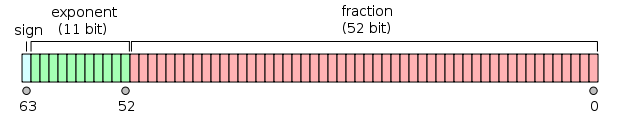
\includegraphics[width=\textwidth]{Double_Floating_Point_Format.png}
			\end{frame}
			
			\begin{frame}
				\frametitle{Floating point arithmetics}
				IEEE 754 standard binary16 (AKA "half" AKA FP16)
				\begin{itemize} 
					\item Sign bit: 1 bit
					\item Exponent: 5 bits
					\item Significand precision: 11 bits (1.xyz)
					\item "3.5" significant decimal digits
				\end{itemize}
				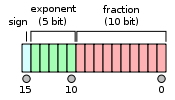
\includegraphics[width=0.3\textwidth]{Half_Floating_Point_Format.png}
				\vspace{\baselineskip}
				4x faster?
			\end{frame}

			\begin{frame}
				\frametitle{Not real numbers arithmetics}
				\begin{itemize} 
					\item limited precission
					\item rounding errors
					\item operations order dependency
					\item under/over-flows
					\item nothing like infinitesimal $\varepsilon > 0, \delta > 0$
				\end{itemize}
			\end{frame}

			\begin{frame}
				\frametitle{NN precision sensitivity - intro}
				\begin{itemize} 
					\item numerical computations (3D physical rendering, simulations ...) usually use FP64 or FP32
					\item NN being succesfully trained on FP16 arithmetic
					\item NN being succesfully deployed on INT8 arithmetic
					\item robust algorithms? empirical evidence...
				\end{itemize}
			\end{frame}
					
	\section{2016 overview}
		
		\subsection{CPU or GPU?}
		
			\begin{frame}
				\frametitle{Performance - benchmarks}
				Benchmarking State-of-the-Art Deep Learning Software Tools\\
				Department of CS, Hong Kong Baptist University, 2017\\
				https://arxiv.org/pdf/1608.07249.pdf\\
				\begin{itemize}
					\item Intel Core i7-3820, Intel Xeon E5-2630
					\item Nvidia GTX 980 (Maxwell), GTX 1080 (Pascal), Tesla K80 (Kepler)
				\end{itemize}
				conclusions
				\begin{itemize}
					\item "GPU is significantly faster." ($\approx$ 10x)
					\item No single best software tool fastest for all tasks.
				\end{itemize}
			\end{frame}
			
			\begin{frame}
				\frametitle{Performance - benchmarks}
				Comparative Study of Deep Learning Software Frameworks\\
				Robert Bosch LLC, 2016\\
				\url{https://arxiv.org/pdf/1511.06435.pdf}\\
				\begin{itemize}
					\item Ubuntu 14.04
					\item Intel Xeon E5-1650 v2 3.50GHz 6Cores HT 
					\item Nvidia GeForce GTX Titan X PCI-E 
				\end{itemize}
				\begin{itemize}
					\item modified LeNet, MNIST dataset\\
						GPU $\approx$ 10x faster
					\item AlexNet, ImageNet dataset\\
						GPU $\approx$ 30x faster
					\item Stacked autoencoders, MNIST dataset\\
						GPU $\approx$ 10x faster
				\end{itemize}
			\end{frame}
			
            \begin{frame}
				\frametitle{Price}
					\begin{itemize}
						\item Intel Core i7-6950X \$1730
						\item Intel Core i7-6900K \$1100
						\item NVidia Titan X (Pascal) \$1200
						\item NVidia GTX 1080 - \$600/700 (founders edition)		
					\end{itemize}
				 \vspace{\baselineskip}
				$\Rightarrow$ Both CPU and GPU price $\approx$ \$1000.
			\end{frame}
            
			\begin{frame}
				\frametitle{Power consumption}
				\begin{itemize}
					\item NVidia Titan X $\approx$ 250W
					\item NVidia GeForce GTX 1080 $\approx$ 180W
					\item Intel Core i7, Xeon $\approx$ 100-140W
				\end{itemize}
			\end{frame}
			
			\begin{frame}
				\frametitle{GPU!}
				\begin{itemize}
					\item price is similar
					\item GPU 10x faster (at least)
					\item GPU power consumption max 2x higher
				\end{itemize}	
				\vspace{\baselineskip}
				...of course system still needs some CPU.
			\end{frame}

		\subsection{General GPU architecture}
        
			\begin{frame}
				\frametitle{GeForce GTX 1080 Block Diagram}
				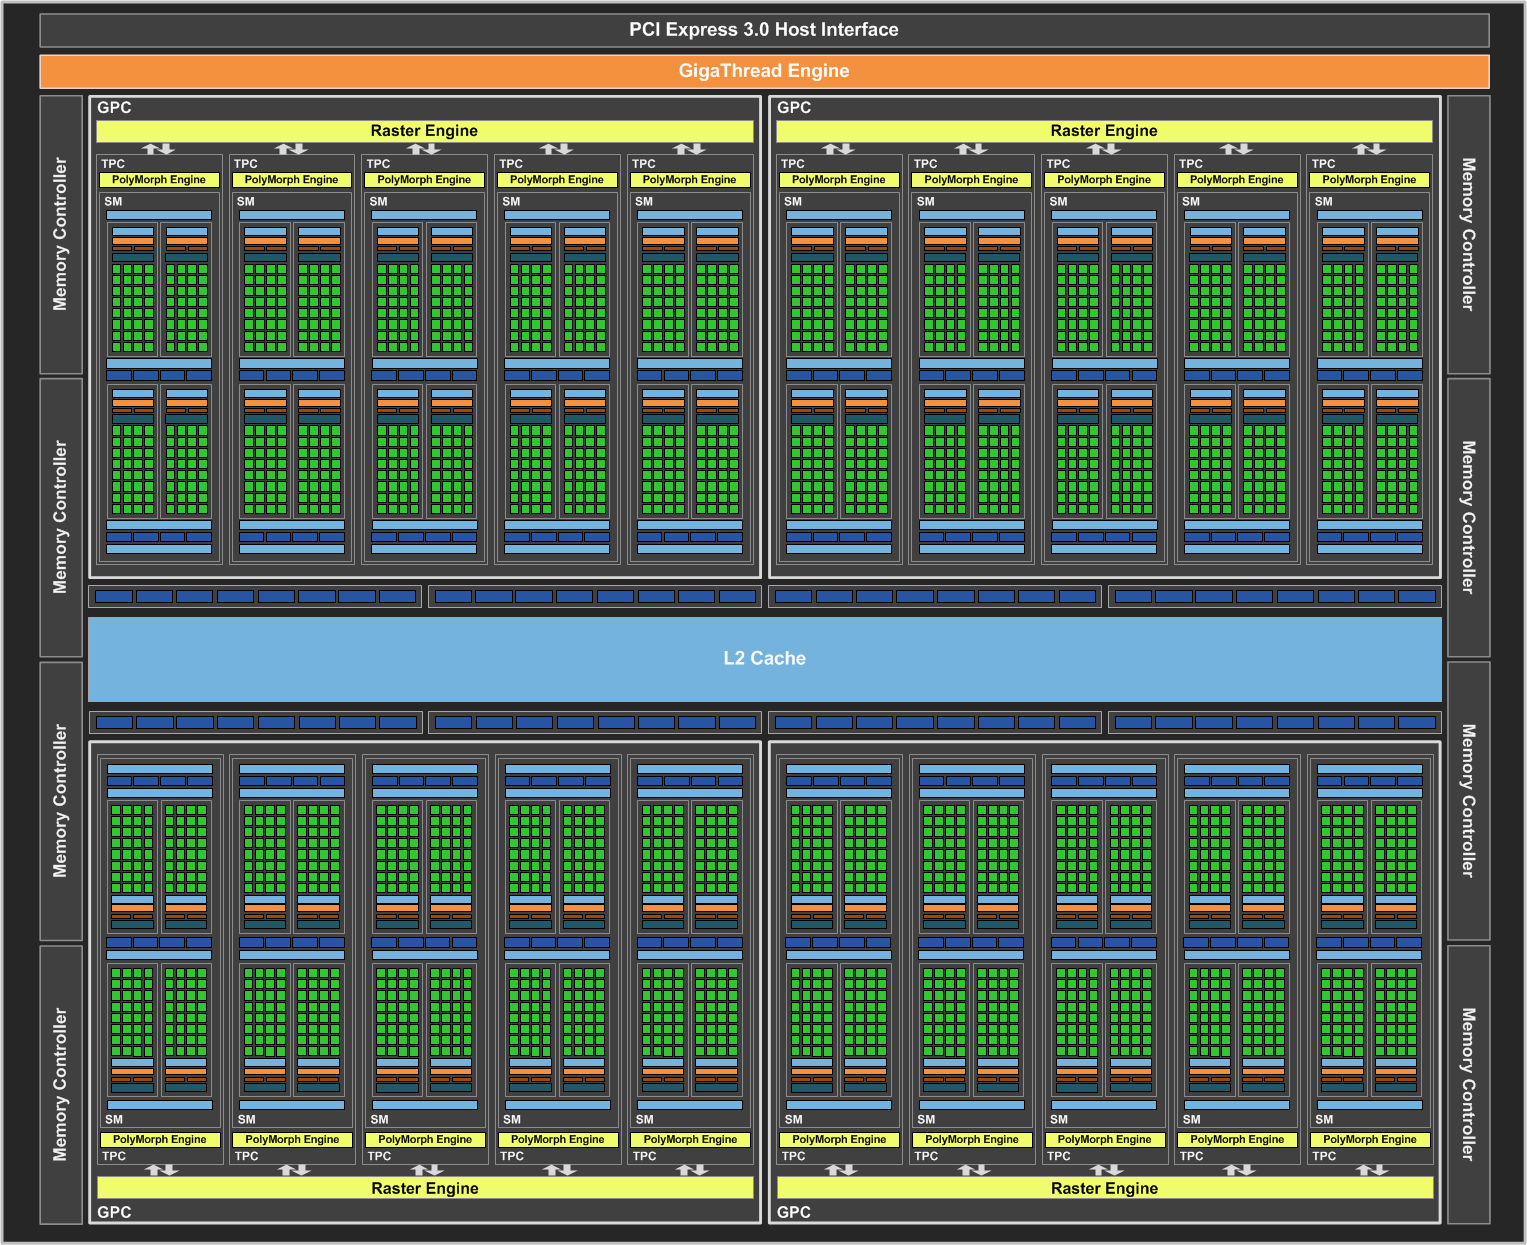
\includegraphics[width=0.8\textwidth]{GeForce_GTX_1080_Block_Diagram_FINAL.png}
			\end{frame}
            
			\begin{frame}
				1 GPU $\approx$
				\begin{itemize}
					\item 10 streaming multi processor
					\item 10 x 100 computational core
					\item 10 x 100 x 10 specific ALU
				\end{itemize}
			\end{frame}
            			
            \begin{frame}
				\frametitle{(definitely NOT) CUDA Core Block Diagram}
				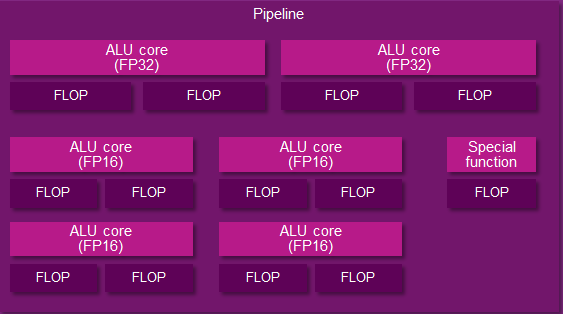
\includegraphics[width=0.8\textwidth]{IMGPipeline.png}
			\end{frame}
            
			\begin{frame}
				\frametitle{Different precision FP arithmetics implementation}
				\begin{itemize} 
					\item Different precision operations are potentially calculated by different ALUs.
					\item Different parts of chip (different transistors) are used for FP64 and FP32 operations.
				\end{itemize} 
			\end{frame}	
            
			\begin{frame}
				\frametitle{GPU Parameters}
				\begin{itemize}
					\item performance [TFLOPS] at optimal precission arithmetic [FP**]
                    \item memory bandwidth [GB/s]
					\item memory size [GB]
					\item power consumption [W]
					\item GPU memory $\leftrightarrow$ CPU memory bandwidth [GB/s]
					\item ...
				\end{itemize}
			\end{frame}
			
			\begin{frame}
				\frametitle{Crucial GPU Parameters?}
				\begin{itemize}
                    \item memory bandwidth [GB/s]
					\item arithmetic performance [TFLOPS] at FP16
				\end{itemize}
                
                For current GPUs bottleneck is memory bandwidth.\\~\\
                For decent utilization of ALUs performance magic is necessary.\\
                Magic is system of memory caches similar to CPU.
			\end{frame}
            
            \begin{frame}
                \frametitle{Naive memory usage}
                GeForce GTX Titan Black (GK110 based)
                \begin{itemize}
                    \item memory bandwidth $\approx$ 0.3TB/s
                    \item FP32 performance $\approx$ 5 TFLOPS
				\end{itemize}
                       
                trivial FP32 $a + b$ with naive memory utilization
                \begin{itemize}
                    \item necessary saturation input:\\
                        $2 \times FP32 \times 5 \times 10^{12} /s = 40 TB/s$
                    \item necessary saturation output:\\
                        $1 \times FP32 \times 5 \times 10^{12} /s = 20 TB/s$
                \end{itemize}
                
                Operation with more input arguments will be even more limited by memory bandwidth.\\
                If performance is plenty FP16 can really be 2x faster than FP32.
            \end{frame}

            \begin{frame}
                \frametitle{Real GPU memory hierarchy}
                NVidia GeForce GTX Titan (Fermi, GK110)
                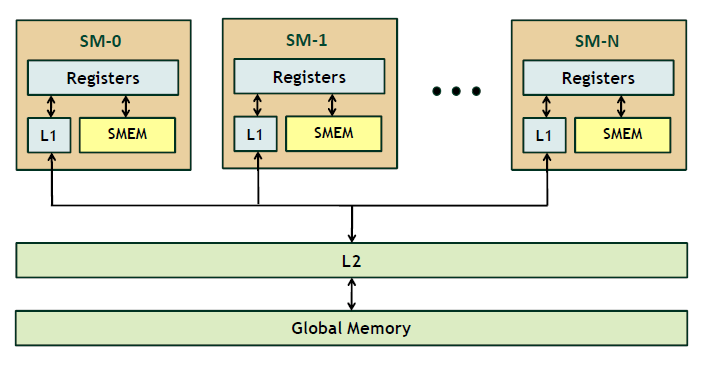
\includegraphics[width=\textwidth]{Fermi_memory_hierarchy.png}
            \end{frame}
            
            \begin{frame}
                \frametitle{Real GPU memory hierarchy bandwidth}
                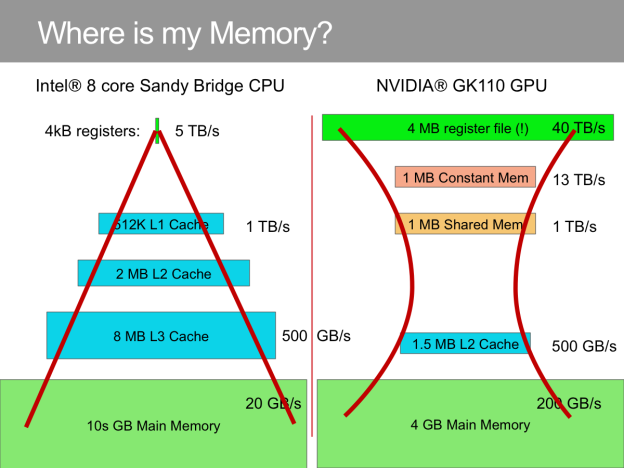
\includegraphics[width=0.8\textwidth]{Fermi_memory_hierarchy_speed_size.png}
            \end{frame}

            \begin{frame}
                \frametitle{Magic}
                    Source:\\
                    \url{http://courses.cms.caltech.edu/cs179/2015_lectures/cs179_2015_lec05.pdf}
                    \begin{itemize}
                        \item Compute throughput: 5 TFLOPS (FP16)
                        \item Global memory bandwidth 336 GB/s (84 G-FP16/s)
                        \item Shared memory bandwidth 3.4 TB/s (853 G-FP16/s)
                    \end{itemize}
                    
                    \begin{exampleblock}{}
                        {\large "If you want to get beyond $\approx$ 900 GFLOPS, need to do multiple FLOPs per shared memory load."}
                    \end{exampleblock}
                    
                    \begin{exampleblock}{}
                        {\large "cuBLAS obtains about 4 TFLOPS on this GPU. Utilization is hard!"}
                    \end{exampleblock}
            \end{frame}

		\subsection{NVidia beats AMD in ML market}

			\begin{frame}
				\frametitle{Similar performance in hardware}
				\begin{itemize} 
					\item AMD Radeon Pro Duo\\
						16.4 TFLOPS @ FP32, HBM (512 GB/s), \$1499, 350W
					\item NVidia GeForce GTX 1080\\
						8.2 TFLOPS @ FP32, GDDR5X (320 GB/s), \$599, 180W
				\end{itemize} 
				\vspace{\baselineskip}
				... ???
			\end{frame}
			
			\begin{frame}
				\frametitle{Low level APIs}
				\begin{itemize} 
					\item OpenCL
						\begin{itemize} 
							\item "Not to be confused with OpenGL"
							\item "Framework for writing programs that execute across heterogeneous platforms consisting of CPUs, GPUs, DSPs, FPGAs and other processors or hardware accelerators."
							\item developed, maintained by Khronos group\\
								(NVidia, AMD, Intel, Apple, Qualcomm, ... + 100)
						\end{itemize} 
					\item CUDA API 
						\begin{itemize} 
							\item "parallel computing platform and programming model"
							\item developed, maintained by NVidia
						\end{itemize} 
				\end{itemize} 
			\end{frame}
			
			\begin{frame}
				\frametitle{ML framework support}
				\begin{itemize} 
					\item OpenCL - Apache Singa, Wolfram Mathematica
					\item CUDA - Keras, TensorFlow, Theano, Torch, ...
				\end{itemize} 
				\begin{itemize} 
					\item NVidia - both OpenCL and CUDA drivers\\
					\item AMD - OpenCL drivers only
				\end{itemize} 
				
				Virtually no support for AMD GPUs by any relevant modern FOSS ML framework.
			\end{frame}
			
		\subsection{NVidia GPU options}
			\begin{frame}
				\frametitle{Pascal architecture}
				Introduced 2016.\\~\\
				
				Two distinct chip categories:
				\begin{itemize} 
					\item "pro" - GP100 chip - Tesla
					\item "consumer/gaming" - GP104 chip - GeForce
				\end{itemize} 
			\end{frame}
			
			\begin{frame}
				\frametitle{GP100 (Tesla)}				
				CUDA core:
				\begin{itemize}
                    \item memory bandwidth 540 (720) GB/s
					\item 64 x FP32 ALU
					\item 0 x FP16 ALU (!?)\\
						vec2 technology - identical operation for 2 inputs of 16bit on single FP32 ALU\\
						for suitable cases as fast as 2x FP16 ALUs
				\end{itemize} 
			\end{frame}	
			
			\begin{frame}
				\frametitle{GP104 (GeForce)}
					CUDA core 
					\begin{itemize} 
                        \item memory bandwidth 480 GB/s
						\item 128 x FP32 ALU
						\item 1 x vec2 FP32 ALU !!!\\
							FP16 performance only 2/128 FP32
                        \item 2x performance in FP32 compared to GP100 constrained by memory bandwidth bottleneck
					\end{itemize} 
					\vspace{\baselineskip}
					???
			\end{frame}
			
			\begin{frame}
				\frametitle{Tesla VS GeForce}				
					
					18.7/21.2 TFLOPS @ FP16 (PCIe/NVLink)
					
					\begin{itemize} 
						\item Tesla P100 PCI-E, 12GB (540GB/s) \$5,899	$\Rightarrow$ \$315/TFLOPS
						\item Tesla P100 PCI-E, 16GB (720GB/s) \$7,374	$\Rightarrow$ \$395/TFLOPS
						\item Tesla P100 SXM2,  16GB (720GB/s) \$9,428	$\Rightarrow$ \$445/TFLOPS
					\end{itemize} 
			
					\begin{itemize} 
						\item GTX 1080: 9 TFLOPS @ FP32 (sic), 8GB (320 GB/s)\\
							\$599 $\Rightarrow$ \$70/TFLOPS (slow? small memory?)
						\item Titan X: 10.2 TFLOPS @ FP32 (sic), 12GB (480 GB/s)\\
							\$999 $\Rightarrow$ \$98/TFLOPS
					\end{itemize} 
					\vspace{\baselineskip} 
					???
			\end{frame}
			
			\begin{frame}
				\frametitle{Why Tesla?}			
					\begin{itemize} 
						\item HBM2?
							\begin{itemize} 
								\item high memory bandwidth
                                \item 256 GB/s memory bandwidth per package, up to 8 GB per package
								\item "slightly" faster than GDDR5X
							\end{itemize} 
                        \item NVLink?
							\begin{itemize} 
								\item CPU-GPU, GPU-GPU interconnect
								\item 20\% theoretical speed-up to PCI-Express
								\item TOP 500 super-computers (proprietary CPU...)
							\end{itemize}
                        \item Avoiding scaling overhead for absolute performance requirements?
					\end{itemize} 
			\end{frame}
			
	\section{2017 news}
		\subsection{AMD ressurection}
		
			\begin{frame}
				\frametitle{New CPU architecture "Zen"}			
				\begin{itemize} 
					\item released March 2nd						
					\item $\approx 50\%$ instructions/clock increase\\
                        (unique for CPU arch in last 5+ years)
					\item $1/2$ - $2/3$ price of comparable Intel CPUs
					\item "ML" branch prediction :-)
				\end{itemize} 
			\end{frame}
			
			\begin{frame}
				\frametitle{New GPU architecture "Vega"}
				\begin{itemize} 
					\item to be released Q2/2017
					\item implemented FP16, FP8 operations
                    \item Vega effect: NVidia GTX 1080 \$599 $\rightarrow$ \$499
					\item GPU MI25
						\begin{itemize}
                            \item HBM2 memory
							\item speculations about 25 TFLOPS @ FP16
							\item (NVidia Titan X : 10.2 TFLOPS @ FP32)
							\item $\Rightarrow$	50TFLOPS @ FP8 ??? ...
						\end{itemize} 
				\end{itemize} 
			\end{frame}
			
			\begin{frame}
				\frametitle{Precission sensitivity of NN learning}
					\begin{itemize}
						\item Deep Learning with Limited Numerical Precision (IBM, 2015)
							\begin{itemize}
								\item "... empirical evaluation ... indicate that in most cases, 8-16 bits of precision is sufficient for back-propagation learning."
								\item custom FPGA + stochastic rounding $\Rightarrow$ 12b fixed pt dec. num. are ok
								\item alternatively start learning with 8bit, finish with 16bit float
								\item https://arxiv.org/pdf/1502.02551.pdf
							\end{itemize} 
						\item Accelerating Deep Convolutional Networks using low-precision and sparsity (Intel, 2016)
							\begin{itemize}
								\item custom FPGA - using CNN with 2bit weights
								\item https://arxiv.org/pdf/1610.00324.pdf
							\end{itemize}
					\end{itemize} 
			\end{frame}
			
			\begin{frame}
				\frametitle{AMD HIP}
					\begin{exampleblock}{}
						{\large "HIP allows developers to convert CUDA code to portable C++."}
						\vskip5mm
						{\large "HIP is very thin and has little or no performance impact over coding directly in CUDA or hcc "HC" mode."}
						\vskip5mm
						{\large "The "hipify" tool automatically converts source from CUDA to HIP."}
						\vskip5mm
						\hspace*\fill{\small--- https://github.com/GPUOpen-ProfessionalCompute-Tools/HIP}
					\end{exampleblock}
			\end{frame}
			
			\begin{frame}
				\frametitle{Radeon Open Compute Platform}
					\begin{exampleblock}{}
					  {\large "With the release of Radeon Instinct, ROCm can accelerate common deep-learning frameworks like Caffe, Torch 7, and TensorFlow on AMD hardware."}
					  \vskip5mm
					  \hspace*\fill{\small--- techreport.com}
					\end{exampleblock}
			\end{frame}
			
			\begin{frame}
				\frametitle{TensorFlow XLA}
					\begin{itemize}
						\item "domain-specific compiler for linear algebra that optimizes TensorFlow computations"
						\item using LLVM backend interface
						\item https://www.tensorflow.org/versions/master/experimental/xla/
					\end{itemize}
			\end{frame}
			
			\begin{frame}
				\frametitle{TensorFlow XLA + ROCm $\overset{?}{=}$ NN @ AMD GPU}
					\begin{exampleblock}{}
						{\large "User Guide for AMDGPU Back-end"}
						\vskip5mm
						\hspace*\fill{\small--- http://llvm.org/docs/AMDGPUUsage.html}
					\end{exampleblock}
					
					\begin{exampleblock}{}
						{\large "Developing a new backend for XLA \\ ... \\ Scenario 2: Non-CPU-like hardware with an existing LLVM backend"}
						\vskip5mm
						\hspace*\fill{\small--- https://www.tensorflow.org }
					\end{exampleblock}
			\end{frame}
            
        \subsection{NVidia strikes back?}
            \begin{frame}
                \frametitle{NVidia 1080 Ti}
                    \begin{itemize}
                        \item announced Feb28, price \$699, GP102 chip
                        \item effectively obsoletes Titan X (only 1GB RAM benefit at \$500 difference)
                        \item FP32 performance $\approx$ 11 TFLOPS
                        \item same design as GTX 1080 (GP104)\\
                            performance @ FP16 is 1/64 performance @ FP32
                        \item GDDR5X memory - bandwidth 484 GB/s
                    \end{itemize}
            \end{frame}
            
	\subsection{NVidia Volta}
        \begin{frame}
            \frametitle{TBA}
                \begin{itemize}
                    \item new NVidia GPU architecture
                    \item rumored to be released 2017-2018
                \end{itemize}
        \end{frame}

\end{document}
